\documentclass[10pt, compress, aspectratio=169]{beamer}

\usetheme[numbering=fraction, progressbar=none, titleformat=smallcaps, sectionpage=none]{metropolis}

\usepackage{sourcecodepro}
\usepackage{booktabs}
\usepackage{array}
\usepackage{listings}
\usepackage{graphicx}
\usepackage[english]{babel}
\usepackage[scale=2]{ccicons}
\usepackage{url}
\usepackage{relsize}
\usepackage{wasysym}
\usepackage{multirow}

\usepackage{pgfplots}
\usepgfplotslibrary{dateplot}

\definecolor{Base}{HTML}{191F26}
\definecolor{Accent}{HTML}{157FFF}

\setbeamercolor{alerted text}{fg=Accent}
\setbeamercolor{frametitle}{bg=Base}

\setsansfont[BoldFont={Source Sans Pro Semibold},
              Numbers={OldStyle}]{Source Sans Pro}

\lstset{ %
  backgroundcolor={},
  basicstyle=\ttfamily\footnotesize,
  breakatwhitespace=true,
  breaklines=true,
  captionpos=n,
  commentstyle=\color{Accent},
  escapeinside={\%*}{*)},
  extendedchars=true,
  frame=n,
  keywordstyle=\color{Accent},
  language=C++,
  rulecolor=\color{black},
  showspaces=false,
  showstringspaces=false,
  showtabs=false,
  stepnumber=2,
  stringstyle=\color{gray},
  tabsize=2,
  keywords={thrust,plus,device_vector, copy,transform,begin,end, copyin,
  copyout, acc, \_\_global\_\_, void, int, float, main, threadIdx, blockIdx,
  blockDim, if, else, malloc, NULL, cudaMalloc, cudaMemcpy, cudaSuccess,
  cudaGetLastError, cudaDeviceSynchronize, cudaFree, cudaMemcpyDeviceToHost,
  cudaMemcpyHostToDevice, const, data, independent, kernels, loop,
  fprintf, stderr, cudaGetErrorString, EXIT_FAILURE, for, dim3},
  otherkeywords={::, \#pragma, \#include, <<<,>>>, \&, \*, +, -, /, [, ], >, <}
}

\renewcommand*{\UrlFont}{\ttfamily\smaller\relax}

\graphicspath{{../img/}}

\title{\textit{OpenMP} or \textit{Pthreads}: \\ Which is Better for Beginners?}
\author{\footnotesize \textbf{Pedro Bruel} {\scriptsize (\textbf{\emph{phrb@ime.usp.br}})} \\
\footnotesize Paulo Meirelles {\scriptsize (\emph{paulormm@ime.usp.br})} \\
\footnotesize Raphael Cobe {\scriptsize (\emph{rmcobe@ncc.unesp.br})} \\
\footnotesize Alfredo Goldman {\scriptsize (\emph{gold@ime.usp.br})}}
\institute{
\includegraphics[height=2cm]{imelogo}\\[0.2cm] \emph{Institute of Mathematics and Statistics} \\ \emph{University of São Paulo}}
\date{\scriptsize PLATEAU, October 23, 2017}

\begin{document}

\maketitle

\section*{Introduction}

%\subsection{About}
%
%\begin{frame}
%    \frametitle{About}
%    \begin{columns}[T,onlytextwidth]
%        \column{0.5\textwidth}
%        \begin{center}
%            
\includegraphics[width=.45\textwidth]{pedro}
%
%            Pedro Bruel \\
%            \emph{\alert{phrb}@ime.usp.br} \\[.3cm]
%            \url{www.ime.usp.br/~phrb} \\
%            \url{github.com/phrb} \\
%        \end{center}
%
%        \column{0.5\textwidth}
%        \begin{center}
%            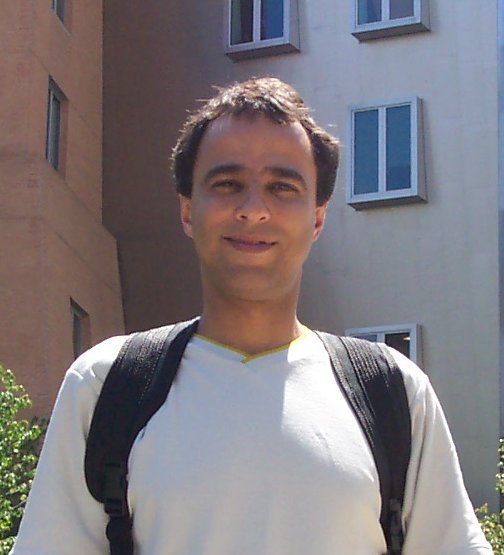
\includegraphics[width=.4\textwidth]{alfredo}
%
%            Alfredo Goldman \\
%            \emph{\alert{gold}@ime.usp.br} \\[.3cm]
%            \url{www.ime.usp.br/~gold} \\
%        \end{center}
%    \end{columns}
%\end{frame}

\subsection*{Outline}

\begin{frame}
    \frametitle{Outline}
    \setbeamertemplate{section in toc}[sections numbered]
    \tableofcontents[hideallsubsections]
\end{frame}

\begin{frame}
    \frametitle{Slides}
    \begin{center}
        
\includegraphics[width=.15\textwidth]{github}
    \end{center}
    The slides, and all data and source code are hosted at \alert{GitHub}:

    \begin{itemize}
        \item \url{github.com/phrb/slides-plateau-2017-which}
        \item \url{github.com/phrb/plateau-2017-which}
    \end{itemize}
\end{frame}

\section{The Course}

\begin{frame}
    \frametitle{The Course}
    The Concurrent, Parallel and Distributed Computing course:

    \begin{itemize}
        \item \alert{Undergraduate} \& \alert{graduate} students in the \alert{same class}
        \item Promote \alert{interaction} between students
        \item More coursework for graduate students
    \end{itemize}

    \pause

    The \alert{objective} is to teach:

    \begin{itemize}
        \item \alert{Core principles} of concurrent, parallel and distributed programming
            \pause
        \item \alert{Hardware fundamentals}: Memory, GPUs, FPGAs
            \pause
        \item Parallel and distributed \alert{programming tools}: \textit{MPI}, \textit{OpenMP}, \textit{Pthreads},
            \textit{CUDA}, $\dots$
    \end{itemize}
\end{frame}

\begin{frame}
    \frametitle{The Classes}
    The classes:

    \begin{itemize}
        \item In \alert{Portuguese}
        \item Professor (Alfredo) \& TA (\alert{Pedro})
        \item Expositions, practical examples \& \alert{programming assignments}
        \item Few non-brazilian students: Iran \& Latin America
    \end{itemize}

    \pause

    With consent from the students, we

    \begin{itemize}
        \item Recorded the classes
        \item Made them available online:
            \url{https://phrb.github.io/MAC5742-0219/aulas.html}
    \end{itemize}
\end{frame}

\begin{frame}
    \frametitle{Students}
    \begin{center}
        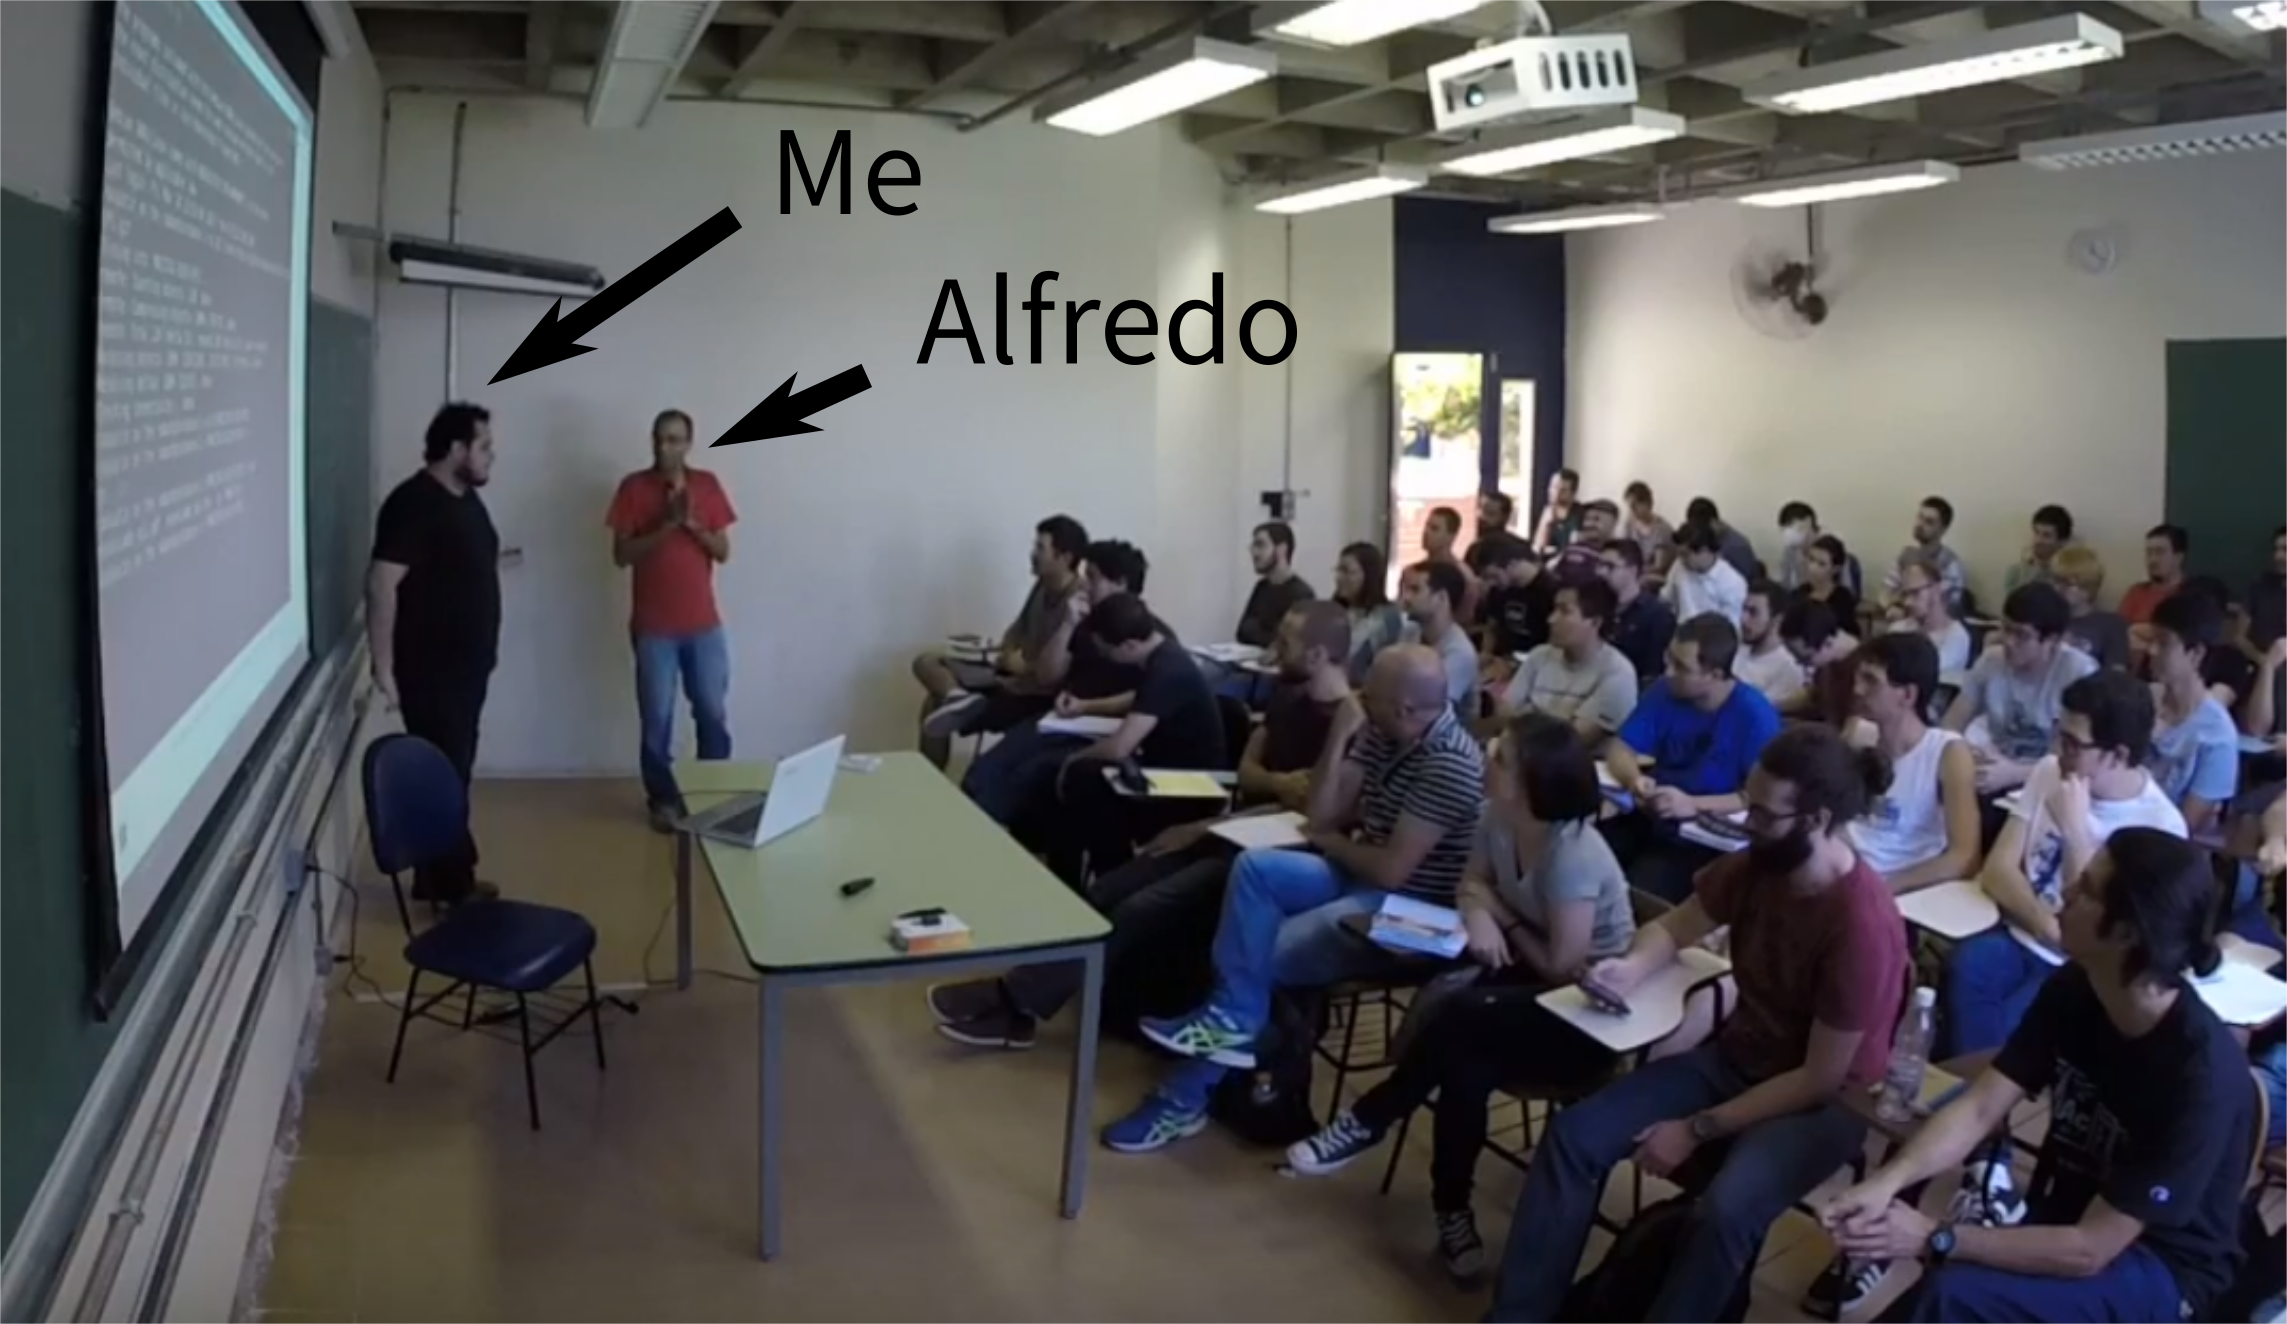
\includegraphics[width=.8\textwidth]{students}
    \end{center}
\end{frame}

\begin{frame}
    \frametitle{Students' Background}
    \begin{center}
        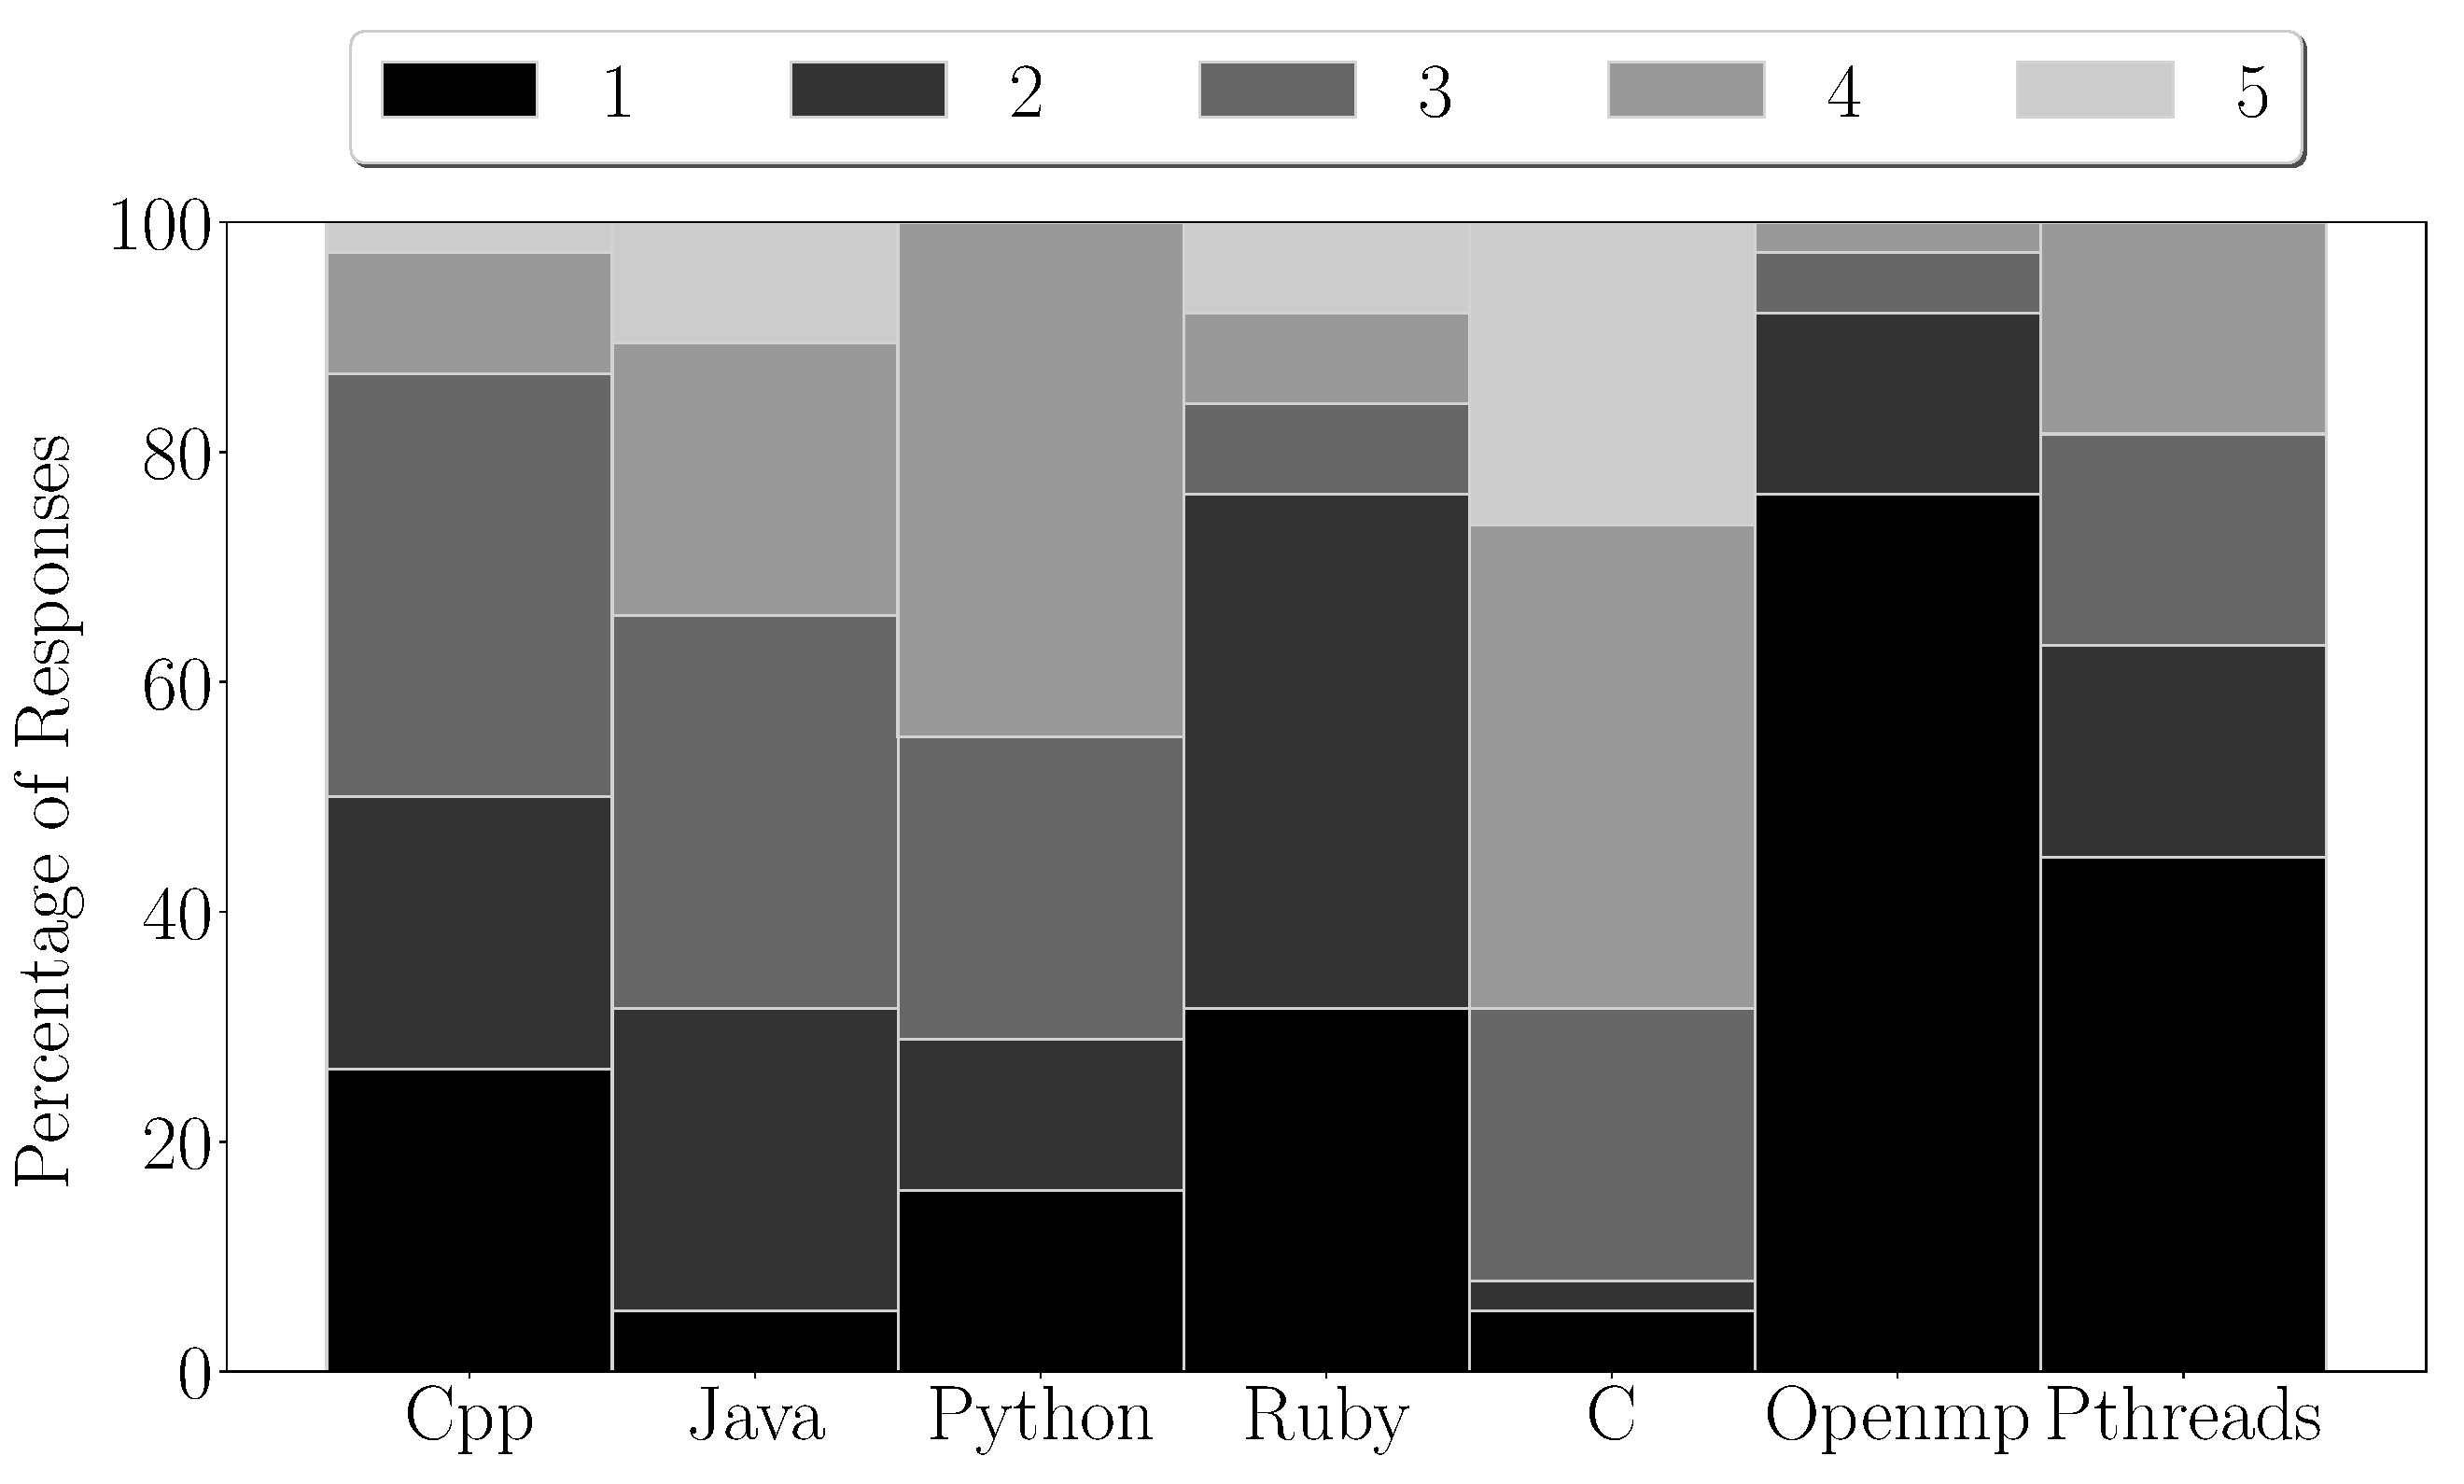
\includegraphics[width=0.78\columnwidth]{background_questions}

        \emph{1: Do not know; 5: Expert}
    \end{center}
\end{frame}

\section{Programming Assignments}

\begin{frame}
    \frametitle{Programming Assignments: Computing the Mandelbrot Set}
    First assignment:

    \begin{itemize}
        \item \alert{Parallelize a sequential version} of the computation of the
            Mandelbrot Set
        \item \alert{Write two versions}, using \textit{OpenMP} and \textit{Pthreads}
        \item \alert{Compare the performance} of the three code versions
    \end{itemize}

    \pause

    \textit{OpenMP}:
    \begin{itemize}
        \item Based on compiler directives
        \item No explicit management required
        \item Usually \alert{considered easier} than \textit{Pthreads}
    \end{itemize}

    \pause

    \textit{Pthreads}:
    \begin{itemize}
        \item Low-level function calls
        \item Explicit management required
        \item Usually \alert{considered harder} than \textit{OpenMP}
    \end{itemize}
\end{frame}

\begin{frame}[fragile]
    \frametitle{Programming Assignments: Computing the Mandelbrot Set}
    \begin{columns}[T,onlytextwidth]
        \column{0.4\textwidth}
        \begin{center}
            
\includegraphics[width=.76\textwidth]{mandelbrot-rotated}
        \end{center}

        \column{0.6\textwidth}
        \begin{center}
            \begin{lstlisting}[language=C, basicstyle=\ttfamily\normalsize, numbers=none,
                   frame=no, showspaces=false, showstringspaces=false,
                   numberstyle=\tiny,
                   xleftmargin=0.1cm,
                   keywords={%
                       DATATYPE, pthread_t, pthread_create,
                       pthread_join, task_function, NULL, int, main,
                       void, printf, return, pthread_mutex_t,
                       pthread_attr_t, pthread_attr_init,
                       MAX_THREADS, SIZE, char, struct, malloc,
                       MIN, pthread_mutex_lock, pthread_mutex_unlock,
                       pthread_exit, from, to, and, for%
                       },
                   otherkeywords={::, \#pragma, \#include, <<<,>>>, \&, \*, +, -, /, [, ], >, <}
                   ]
z = 0;
for(x from 0 to x_max - 1) {
  /* Independent iterations */
  for(y from 0 to y_max - 1) {
    /* Independent iterations */
    for (iteration from 0 to
         iteration_max,
         and f_c(z) < limit) {
      z = f_c(z);
      /* Iterations depend on
         previous values of z */
    }
  }
}
            \end{lstlisting}
        \end{center}
    \end{columns}
\end{frame}

\begin{frame}
    \frametitle{Other Assignments}
    Other assignments:

    \begin{itemize}
        \item Parallelize crypto algorithms using CUDA
        \item Distributed Mandelbrot using the Google Compute Engine
    \end{itemize}
\end{frame}

\section{Questionnaire \& Responses}

\begin{frame}
    \frametitle{Research Questions}
    In our first study, published at HICSS 2017, students helped us show that
    \alert{OpenMP is not as easy as it appears}.

    \pause

    Now, we wanted to know:

    \begin{description}
        \item[RQ1:] \textit{According to the students' perception, which API was
            easier to learn and use?}
        \item[RQ2:] \textit{With which API did the students improve performance the
            most?}
        \item[RQ3:] \textit{Did the students' performance improvements match their
            perception?}
    \end{description}
\end{frame}

\begin{frame}
    \frametitle{The Questionnaire}
    Measure the students' \alert{subjective perceptions} of \textit{Pthreads}
    and \textit{OpenMP}:

    \begin{itemize}
        \item Independently
        \item Relative to each other
    \end{itemize}

    \pause

    \textit{We had approval from our University's Ethics Board, and consent
    from individual students}
\end{frame}

\begin{frame}
    \frametitle{Independent Questions: RQ1 \& RQ2}
    \begin{columns}[T,onlytextwidth]
        \column{0.4\textwidth}
        \begin{table}
            \centering
            \begin{tabular}{@{}p{0.65\columnwidth}p{0.18\columnwidth}p{0.05\columnwidth}@{}}
                \toprule
                \multicolumn{2}{c}{\normalsize{It is easy to$\dots$}} & \textnumero \\ \midrule
                \multirow{2}{*}{\parbox{0.7\columnwidth}{\normalsize{Parallelize loops with independent iterations using:}}} & \normalsize{OpenMP} & $(1)$ \\
                & \normalsize{Pthreads} & $(2)$ \\ \addlinespace \addlinespace
                \multirow{2}{*}{\parbox{0.7\columnwidth}{\normalsize{Parallelize nested loops with independent iterations using:}}} & \normalsize{OpenMP} & $(3)$ \\
                &  \normalsize{Pthreads} & $(4)$ \\ \addlinespace \addlinespace \addlinespace
                \multirow{2}{*}{\parbox{0.7\columnwidth}{\normalsize{Improve the performance of sequential code using:}}} & \normalsize{OpenMP} & $(5)$  \\
                &  \normalsize{Pthreads} & $(6)$ \\ \bottomrule
            \end{tabular}
        \end{table}

        \column{0.6\textwidth}
        \begin{center}
            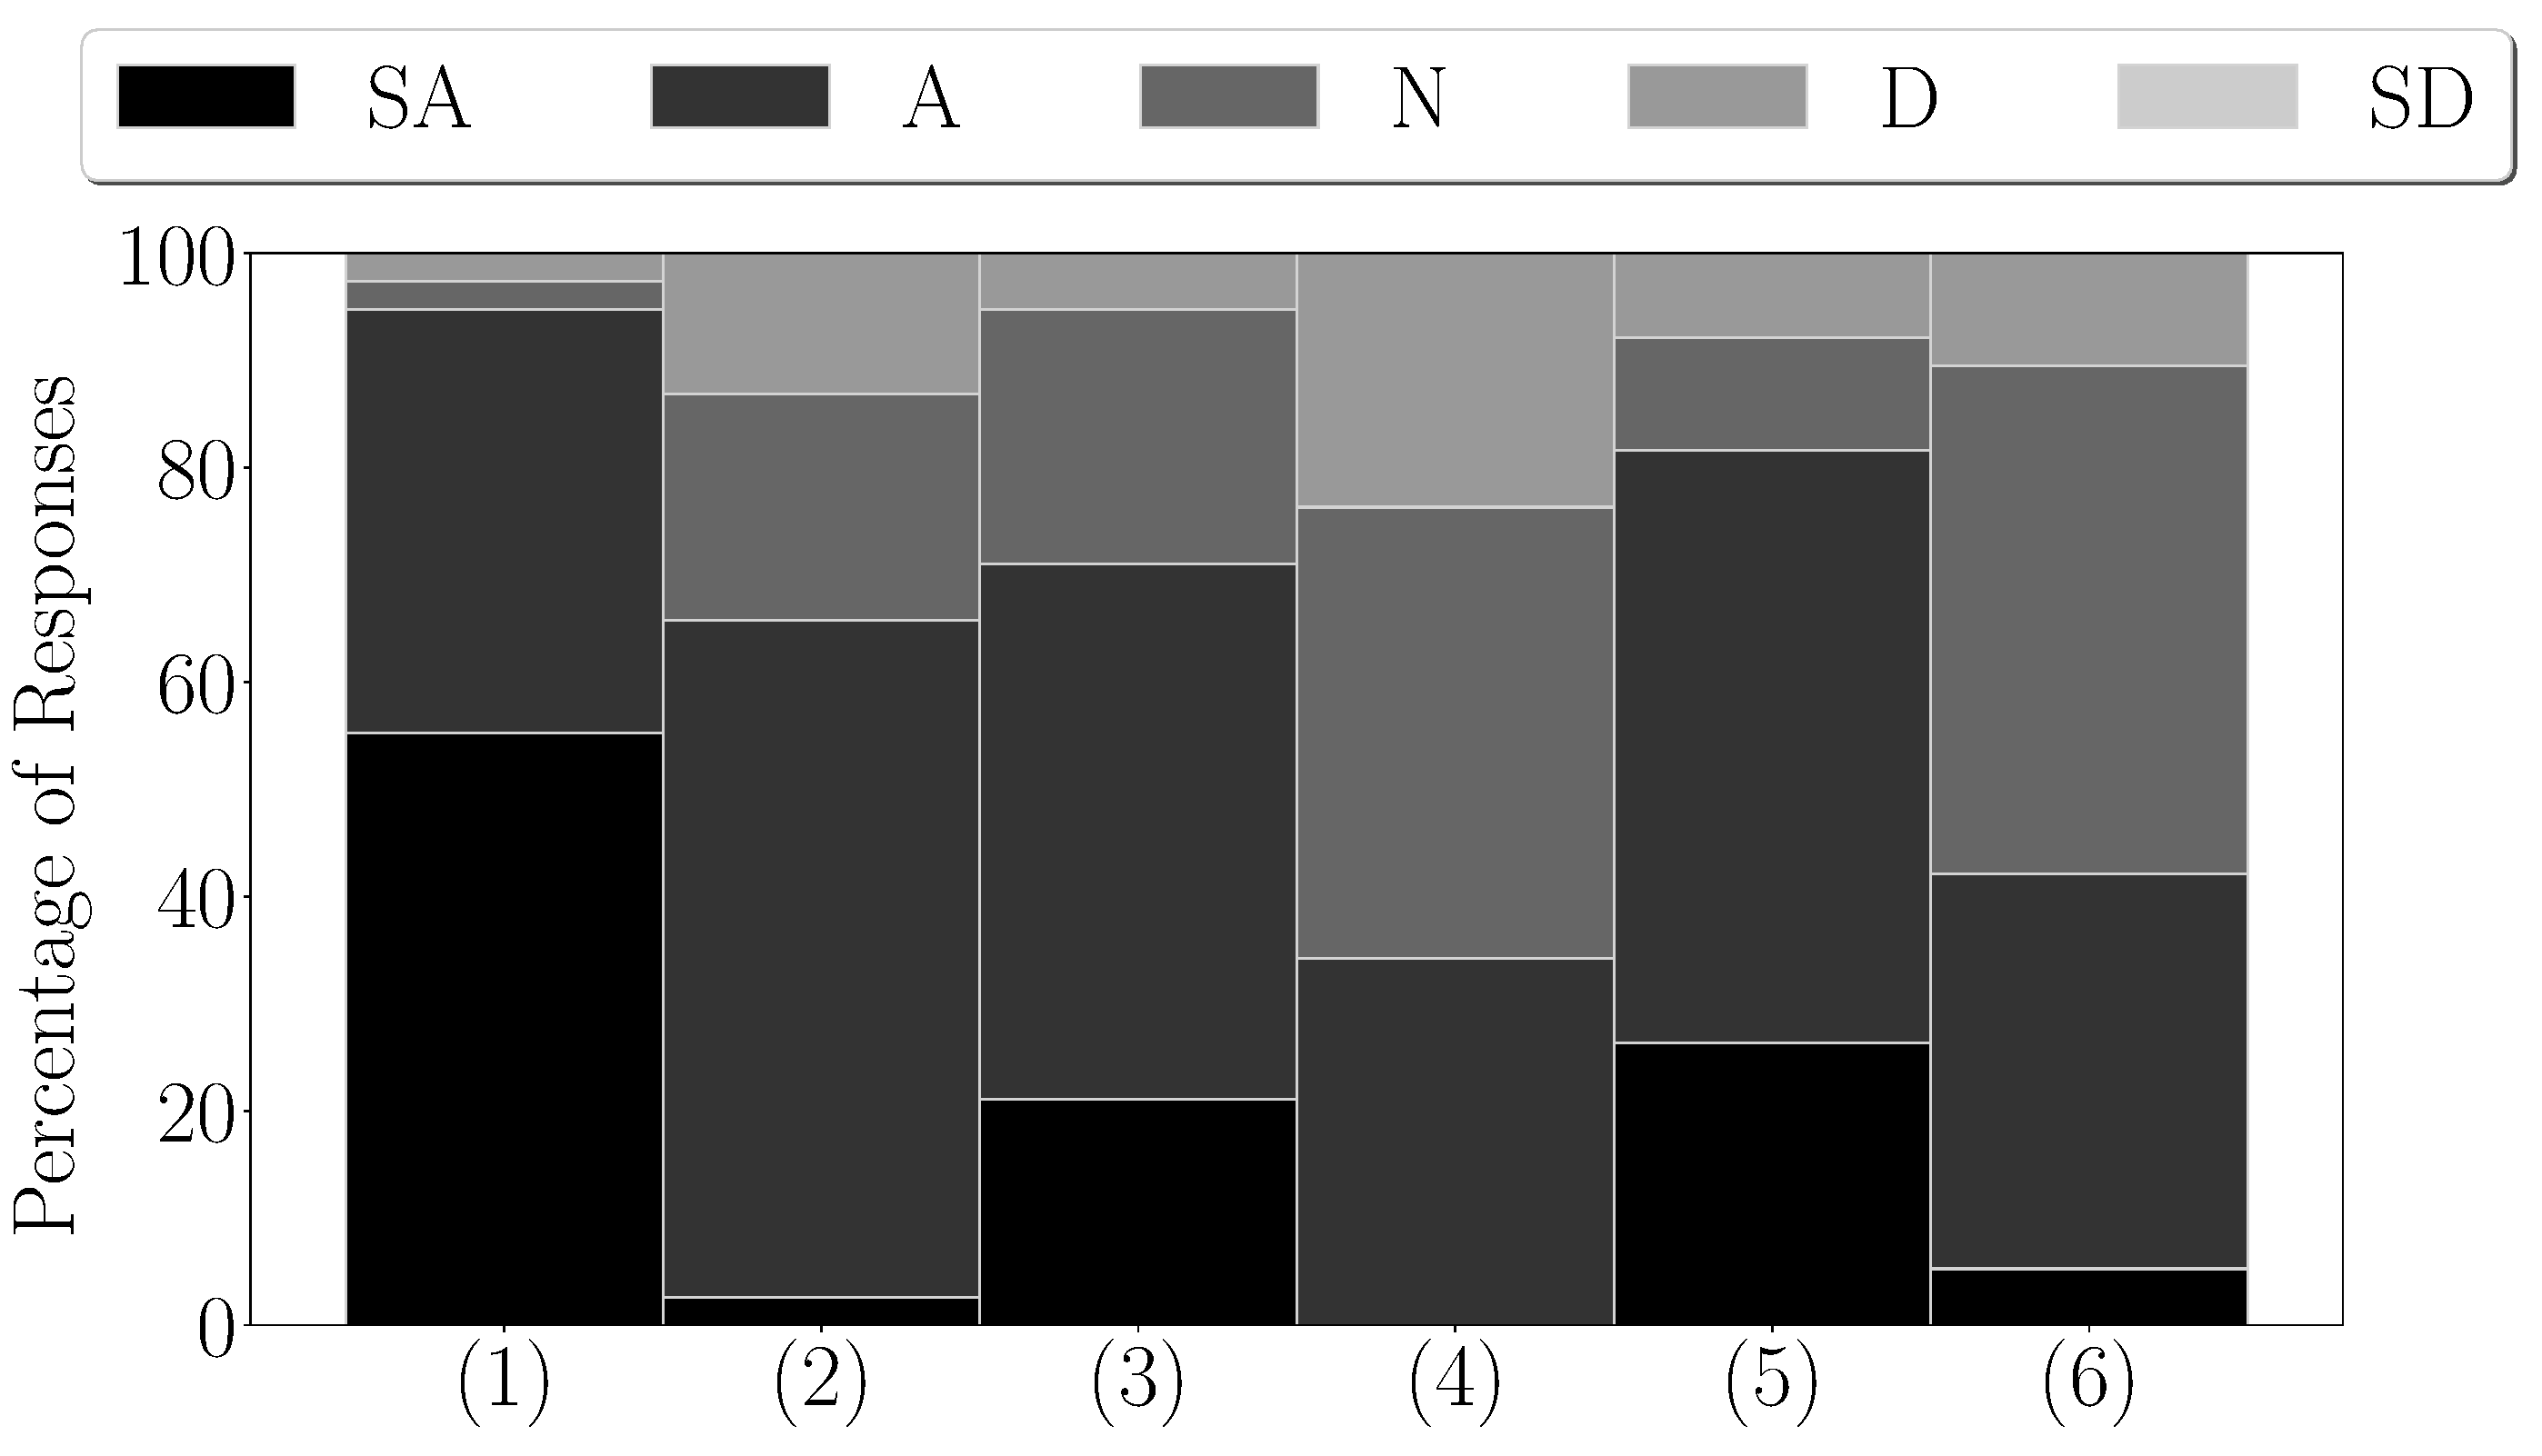
\includegraphics[width=0.85\columnwidth]{likert_questions}

            \emph{SA: Strongly Agree; SD: Strongly Disagree}
        \end{center}
    \end{columns}
\end{frame}

\begin{frame}
    \frametitle{Comparison Questions: RQ2 \& RQ3}
    \begin{columns}[T,onlytextwidth]
        \column{0.4\textwidth}
        \begin{table}
            \centering
            \begin{tabular}{@{}p{0.9\columnwidth}p{0.08\columnwidth}@{}}
                \toprule
                \multicolumn{1}{c}{\footnotesize{Which technology$\dots$}} & \textnumero \\ \midrule
                \footnotesize{Was more difficult to learn?} & $(7)$ \\ \addlinespace
                \footnotesize{Was simpler to use?} & $(8)$ \\ \addlinespace
                \footnotesize{Was easier to use?} & $(9)$ \\ \addlinespace
                \footnotesize{Was easier to use for parallelizing loops with independent iterations?} & $(10)$ \\ \addlinespace
                \footnotesize{Was easier to use for parallelizing nested loops with independent iterations?} & $(11)$  \\ \addlinespace
                \footnotesize{Was easier to use for improving the performance of a sequential program?} & $(12)$  \\ \addlinespace
                \footnotesize{\alert{Had the best performance on your assignment?}} & \alert{$(13)$} \\ \bottomrule
            \end{tabular}
        \end{table}

        \column{0.6\textwidth}
        \vspace{1cm}
        \begin{center}
            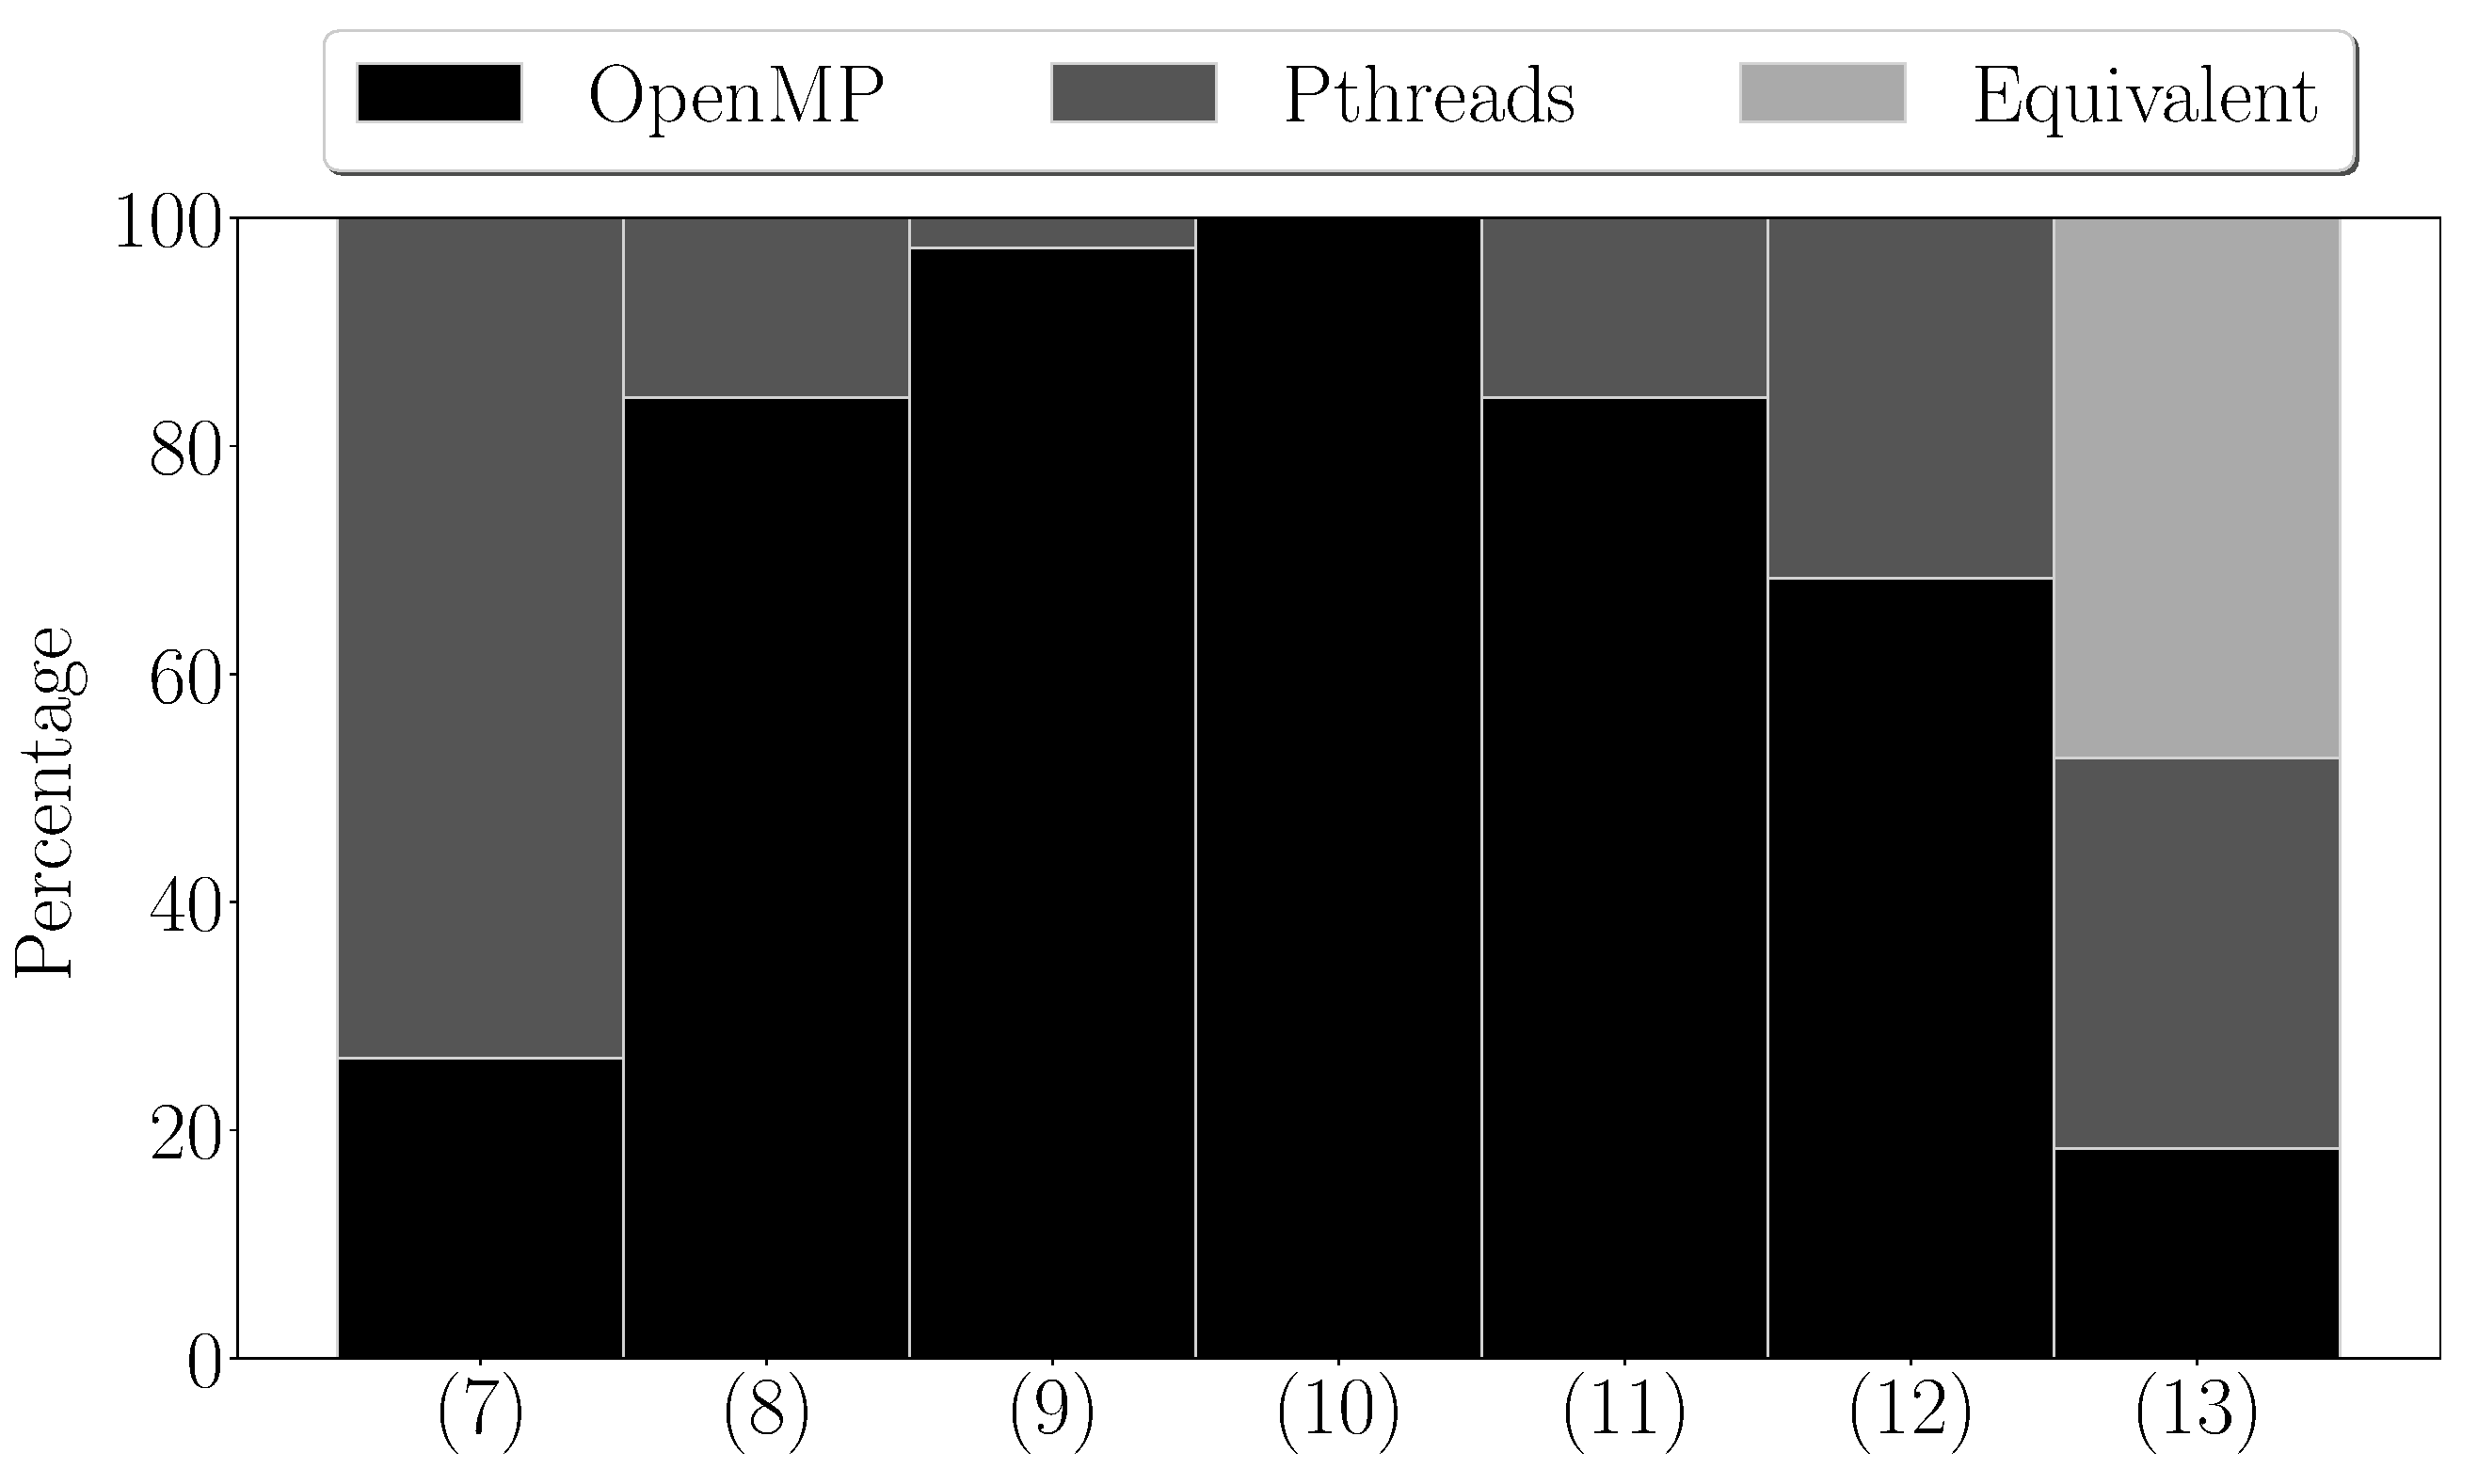
\includegraphics[width=0.85\columnwidth]{comparisons}
        \end{center}
    \end{columns}
\end{frame}

\begin{frame}
    \frametitle{Conclusion}
    We conclude that:

    \begin{itemize}
        \item The \alert{students' perceptions did not match} the performance they
            achieved
        \item \textit{OpenMP} is still not as easy as it appears
        \item Students are capable of achieving \alert{better performance} with
            \alert{lower-level} parallel programming APIs
    \end{itemize}
\end{frame}

\section{Threats to Validity}

\begin{frame}
    \frametitle{Threats to Validity}
    \alert{Threats to validity} include:

    \begin{itemize}
        \item Study performed in a \alert{single instance of the course}
            \pause
        \item No \alert{control group} or separate groups
            \pause
        \item \alert{Subjectivity} of questionnaire and responses
    \end{itemize}

    \pause

    We will continue this research and seek to eliminate these threats
\end{frame}

\maketitle

\end{document}
